\chapter{Omówienie problemu}

\section{Czym są fiszki?}

Nauka z wykorzystaniem metody fiszek opiera się na systemie regularnych powtórek rozłożonych w czasie. Jest jednym z najpopularniejszych i najbardziej efektywnych sposobów pozwalających przyswoić i utrwalić wiedzę. Technika ta w klasycznej wersji polega na regularnym dobieraniu kart z talii, w której wszystkie są zapisane z dwóch stron – na jednej stronie każdej fiszki znajduje się zagadnienie, na drugiej, natomiast przeznaczone do zapamiętania klucz odpowiedzi lub definicja. Karty są dobierane z talii kolejno w sposób losowy, po każdorazowym dobraniu należy odczytać zagadnienie lub kłopotliwy termin, a następnie spróbować odpowiedzieć zgodnie z kluczem zapisanym na drugiej stronie. Wtedy dopiero można dokonać porównania i zestawić swoją odpowiedź z prawidłową, zapisaną na odwrocie fiszki. Następnie, karta powinna wrócić do talii, tj. zbioru.

Rozwój technologiczny oraz dobiegająca zewsząd cyfryzacja powoli wypierają z użytku klasyczną formę stosowania fiszek na rzecz jej organizacji poprzez aplikacje mobilne oraz strony internetowe. Zmiana ta niesie wiele szans oraz możliwości udoskonalenia metody fiszek w jej skuteczności oraz dostępności. Fundamentalną zmianą jest samo przyśpieszenie całego procesu sporządzania talii oraz ich przeglądania – przy wykorzystaniu komputera lub smartfonu staje się to znacznie prostsze i szybsze niż ręczne zapisywanie kart, wycinania ich i gromadzenie.

\section{Przedstawienie problemu}

Celem projektu jest zwiększenie efektywności uczenia się metodą fiszek poprzez jej integracje z interfejsem bezdotykowym. Pomimo dużego wkładu w przystępność i zwiększenie dostępności tej metody przez cyfrowe rozwiązania, istniejące aplikacje do tworzenia i przeglądania fiszek wymagają zasadniczo aktywnego zaangażowania użytkownika poprzez klikanie lub wpisywania na klawiaturze – zarówno przy użyciu smartfonów, jak i komputerów osobistych. Ta konieczność bezpośredniej interakcji ogranicza możliwości nauki do określonych sytuacji, co stanowi barierę w momentach, gdy użytkownik wykonuje inne czynności, na przykład proste prace domowe, a urządzenie obsługujące aplikacje nie może być efektywnie wykorzystane.

Dodatkowo proces tworzenia fiszek, który wymaga od użytkowników manualnego redagowania, przepisywania lub kopiowania definicji, znacząco opóźnia przygotowanie materiałów do nauki i wydłuża czas potrzebny na stworzenie talii kart. Ta czasochłonna procedura potrafi stanowić istotną przeszkodę, ograniczając proces uczenia się. Czas, który mógłby być przeznaczonym na utrwalanie wiedzy, jest poświęcany na przygotowanie zasobów służących do nauki. Sama potrzeba redagowania fiszek może odebrać użytkownikowi chęci by w ogóle korzystać z tej metody. Celem projektu jest częściowa automatyzacja procesu tworzenia talii poprzez wzbogacenie funkcjonalności o narzędzia sztucznej inteligencji. Skutkiem tego jest możliwość generowania kluczy odpowiedzi fiszek odpowiednio do podanych zagadnień.

W odpowiedzi na te wyzwania, opisany w niniejszej pracy system dąży do zminimalizowania ograniczeń związanych z tradycyjną obsługą aplikacji oferujących możliwość nauki metodą fiszek. Podjęty projekt proponuje rozwiązanie, które integruje proces przyswajania wiedzy z codziennymi czynnościami użytkownika oraz umożliwia jednocześnie szybsze i bardziej intuicyjne tworzenie materiałów do nauki. Celem realizowanego projektu jest stworzenie aplikacji, w której nauka jest nie tylko bardziej efektywna, ale również dostępna w szerokim zakresie sytuacji z pomocą bezdotykowej obsługi.


Poniżej znajduje się graficzna reprezentacja problemu ujętego w formie Rich Picture:
\begin{figure}[H]
    \centering
    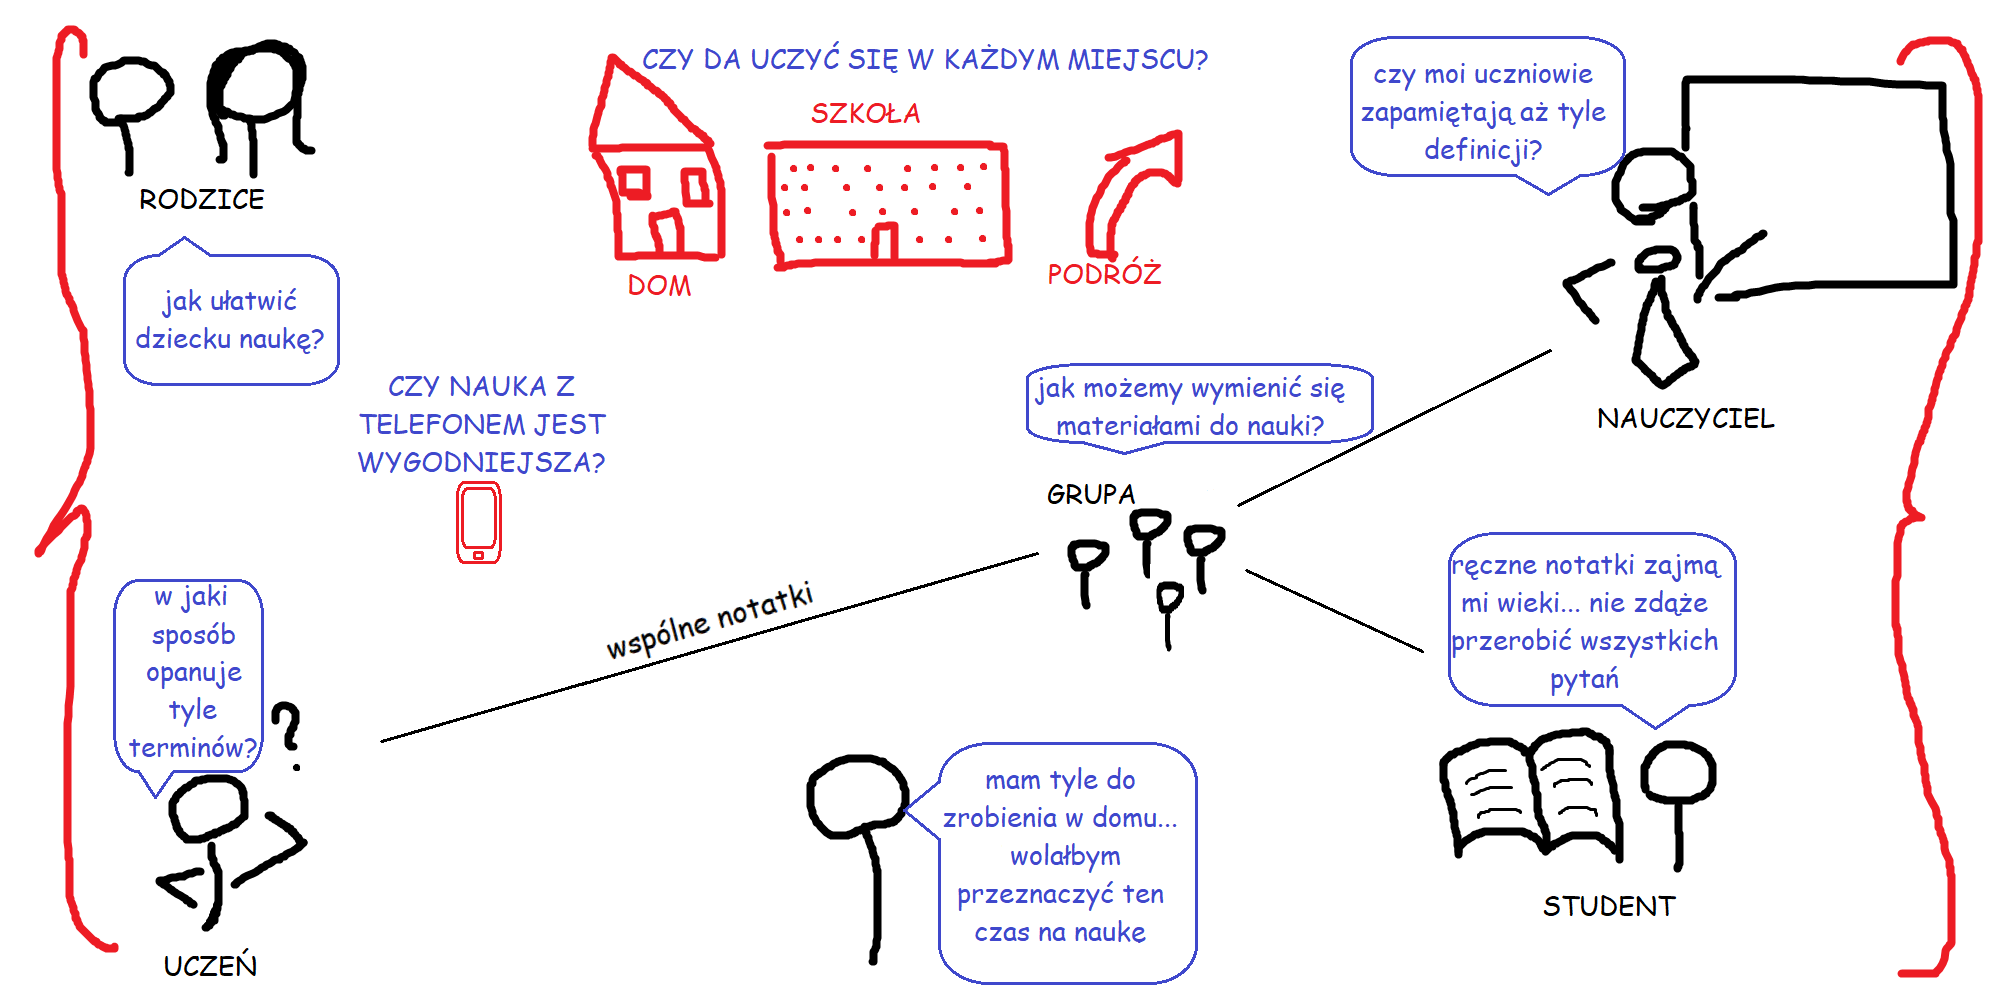
\includegraphics[width=1\textwidth]{chapters/chapter_2/rich_picture.png}
    \caption{Problem przedstawiony w rich picture.}
    \label{img:rich_picture}
\end{figure}


\section{Zalety nauki z wykorzystaniem metody fiszek}

Nauka z wykorzystaniem fiszek to jedna z najbardziej popularnych i elastycznych metod. Dzięki jej prostocie i skuteczności znajduje zastosowanie w różnych kontekstach edukacyjnych. W poniższym podrodziale szczegółowo przyjrzymy się mechanizmowi, dzięki któremu fiszki tak skutecznie wspierają proces nauki.


\subsection{Krzywa zapominania Hermanna Ebbinghausa}

Opierając się na systemie regularnych powtórek, praktykowana metoda fiszek pozwala na utrzymanie stanu wiedzy na wysokim poziomie zgodnie z zasadami krzywej zapominania Ebbing hausa. Mowa o zależności opisanej przez niemieckiego psychologa, Hermanna Ebbing hausa. Według wyników badań opublikowanych w 1885 roku w pracy "Uber das Gedächtnis"\cite{ebbinghausMemoryCurve}  (w tłumaczeniu „O pamięci”), najlepszym sposobem na zapamiętanie jest rozłożenie nauki w czasie. Praktyka ta jest znacznie skuteczniejsza od skupienia nauki w jednym okresie. Istotnym elementem zagadnienia jest wykres omawianej krzywej:

\begin{figure}[H]
    \centering
    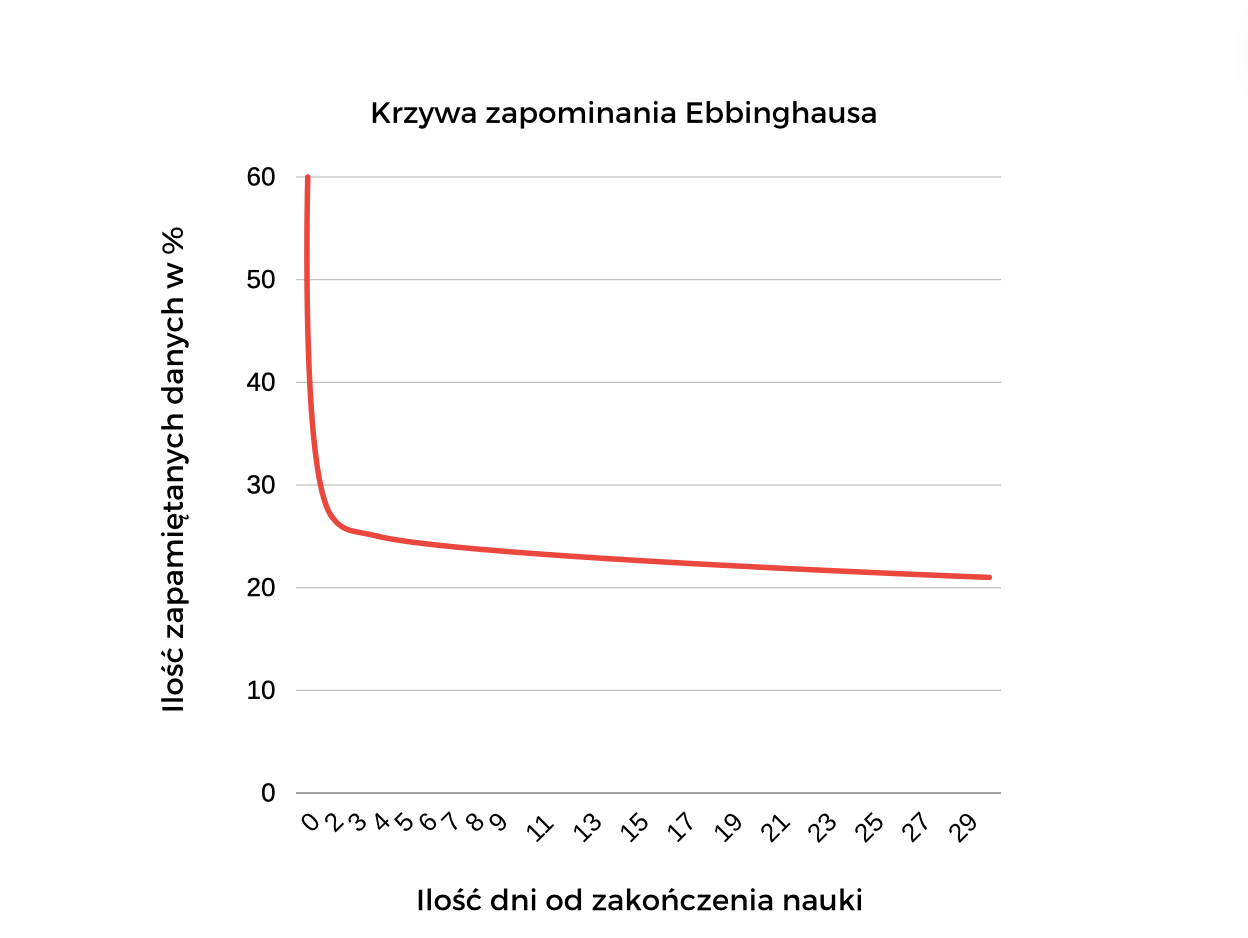
\includegraphics[width=0.8\textwidth]{chapters/chapter_2/krzywa1.png}
    \caption{Wizualizacja wyniku badań Ebbinghausa.}
    \label{img:krzywa1}
\end{figure}

Powyższy wykres reprezentuje tempo, w którym następuje zapominanie nauczonych treści po zakończeniu nauki. W przeciągu pierwszych kilku dni od jej zakończenia następuje gwałtowny spadek zapamiętanych informacji, nawet do poziomu 25\% względem całkowitej ilości powtarzanych informacji. Dopiero po upływie tego czasu krzywa się stabilizuje, a tempo zapominania znacznie zwalnia. Najskuteczniejszym według badania sposobem by zapobiec temu procesowi jest regularne powtarzanie materiału. Poniższy wykres przedstawia ilość przyswojonej wiedzy względem każdej kolejnej sesji nauki:

\begin{figure}[H]
    \centering
    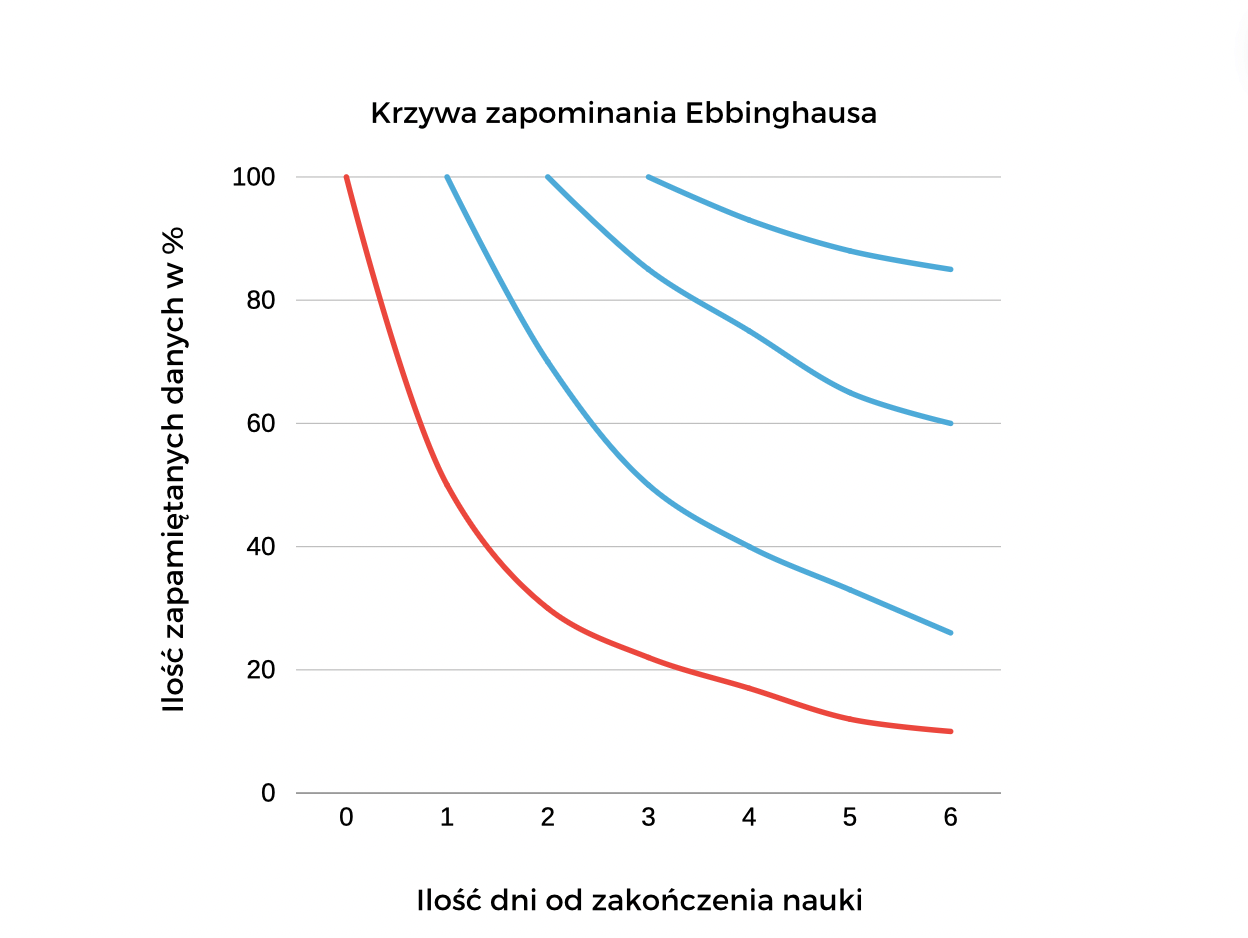
\includegraphics[width=0.8\textwidth]{chapters/chapter_2/krzywa2.png}
    \caption{Wizualizacja wyniku badań Ebbinghausa.}
    \label{img:krzywa2}
\end{figure}


Przyjmuje się, że metoda nauki z regularnymi powtórkami, jaką oferuję metoda fiszek, pozwala na skuteczne utrwalenie wiedzy i znaczne spowolnienie zapominania jej. Użyte w badaniu informacje, które zostały podjęte nauce były danymi „bezużytecznymi”. Hermann Ebbinghaus celowo używał losowo utworzonych sylab, aby zminimalizować zależności między danymi a osobami, które się uczyły. Powszechnie akceptowane w psychologii edukacyjnej jest twierdzenie, że przyswojenie informacji, które indywidualnie uznaje się za jakikolwiek interesujące dodatkowo ułatwia proces ich zapamiętania. Idące za tym wnioski plasują metodę regularnych powtórek jako tym bardziej przystępna, ponieważ znajduje zastosowanie nawet w przypadku zapamiętywania informacji, które niekoniecznie muszą być dla odbiorcy atrakcyjne.

\subsection{Przykłady praktycznych zastosowań fiszek}

Metoda nauki z wykorzystaniem fiszek znajduje szerokie zastosowanie w różnych dziedzinach nauki i życia codziennego, jej przystępna forma odpowiada poniższym przykładom:
\begin{itemize}
    \item Nauka języków obcych: fiszki są powszechnie stosowane w celu utrwalenia słownictwa, zwrotów lub zasad gramatycznych języków obcych; szybkie przypominanie i testowanie wiedzy jest w tym przypadku kluczowe w procesie opanowywania języka innego niż ojczysty;
    \item Nauki techniczne: ze względu na dużą ilość szczegółowych informacji, które istotnie trzeba spamiętać, fiszki są odpowiednim narzędziem dla studentów lub pracowników branży technicznych. Pomagają one w efektywnym przyswajaniu skomplikowanych terminów;
    \item Przygotowanie do egzaminów: uczniowie i studenci przygotowujący się do egzaminów mogą wykorzystać fiszki w celu opanowania kluczowych pojęć, definicji czy zestawu odpowiedzi.
\end{itemize}

\subsection{Personalizacja fiszek}

Do najważniejszych zalet nauki metodą fiszek zalicza się możliwość personalizacji materiałów naukowych. Osoby korzystające z fiszek mogą tworzyć własne talie, dostosowane do ich indywidualnych potrzeb i preferencji. Dodatkowo fiszki mogą być łatwo dostosowane do różnych sposobów uczenia się, przykładowo poprzez stosowanie trybu obsługi głosowej.

\section{Słownik pojęć}

\begin{enumerate}
    \item Fiszka - karta zapisana z dwóch stron, na jednej stronie znajduje się pytanie/zagadnienie, na drugiej odpowiedź/definicja.
    \item Talia - zbiór, pula fiszek.
    \item System - przedmiot projektu, ogólne określenie wytworzonej aplikacji mobilnej, webowej.
    \item Gamifikacja/Grywalizacja - wykorzystanie elementów gier w niezwiązanym z grami kontekście.\cite{gamificationWiki}
    \item Model nlp - zastosowany w projekcie moduł rozpoznawania i analizy instrukcji głosowych.
    \end{enumerate}
